\subsection{Pipeline Architecture Improvements}

We identify several complementary directions for improving the oracle pipeline that extend its retrieval, evidence selection, and aggregation layers. Figure~\ref{fig:future_system} illustrates the proposed modifications.

\subsubsection{Specialized Retrieval for Domain-Specific Questions}

A recurring source of error in our evaluation was questions requiring precise, structured data that general-purpose search engines are poorly suited to retrieve. For example, a question such as "Will the price of Bitcoin be above \$80,000 on March 24th, 2025?" requires a single authoritative price observation at a specific timestamp. This information is trivially available through a cryptocurrency price API like CoinGecko but difficult to extract reliably from web search results, which may return commentary, forecasts, or prices from neighboring dates. Our use of Exa as a uniform retrieval backend for all question types meant that such domain-specific queries often received evidence packets that were insufficient for confident resolution. A more robust system would combine a general-purpose retrieval layer for open-ended questions with specialized API integrations dispatched based on question category or content. For categories like Crypto or Financials, a routing layer could detect that the question requires a structured data lookup and query the appropriate domain API directly, using cheap and deterministic lookups for questions that warrant them and general search for everything else.

\begin{figure}[t]
    \centering
    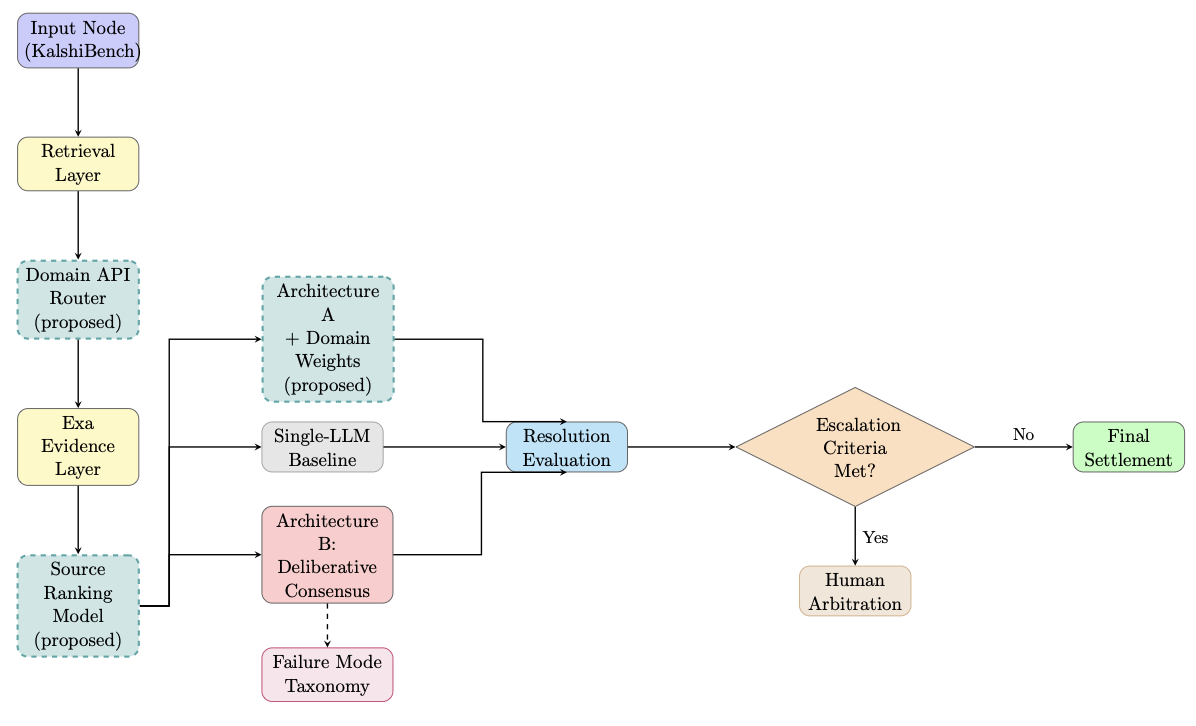
\includegraphics[width=\linewidth]{figures/figure7_proposed_future_system.png}
    \caption{\textbf{Extended system flow with proposed future-work updates.} 
    The pipeline introduces domain-specific retrieval routing, learned source ranking, and domain-aware aggregation to improve retrieval quality, evidence prioritization, and ensemble performance.}
    \label{fig:future_system}
\end{figure}


\subsubsection{Source Quality Weighting and Learned Source Ranking}

Our current pipeline treats all retrieved sources equally, passing the same unweighted evidence packet to every agent. However, not all sources are equally informative or reliable for a given question: a primary government data release carries more evidentiary weight than a speculative blog post. A natural extension would be to introduce a learned source-ranking layer that scores and weights retrieved documents before they reach the resolution agents. One promising approach would train an embedding model to reproduce quality rankings generated by LLM judges applied to oracle resolution traces. Specifically, for a set of resolved questions with known ground-truth outcomes, one could use one or more LLM judges to rank the sources in each evidence packet by their contribution to a correct resolution. These ranked preferences would then serve as training signal for a lightweight source-ranking model that could be applied at inference time without the cost of repeated LLM judge calls. Evaluation of such a system is straightforward in principle. By holding the resolution architecture fixed, one can measure whether accuracy improves when agents receive source-weighted evidence compared to the uniform-weight baseline used in this study. Beyond accuracy, source weighting could also improve calibration by allowing agents to express lower confidence when their highest-weighted sources are weak, providing a more informative signal for the escalation framework developed in this thesis.

\subsubsection{Principled Abstention as a Third Resolution Output}

Our current agent schema forces a binary decision. Every agent must output YES or NO for every question, regardless of evidence quality. While agents can express low confidence, they cannot explicitly signal that the evidence is insufficient to resolve the question. This constraint is a direct contributor to several failure modes identified in Section~\ref{sec:failure}. In retrieval failures, agents produce confident but wrong answers because the evidence packet appears substantive even when the critical piece of information is absent. In temporal reasoning errors, agents correctly recognize that their evidence contains only forecasts rather than observed outcomes, but are forced to pick a side rather than flag the evidence gap.

Adding abstention changes the aggregation logic in meaningful ways. Under the current majority-vote scheme, a 2-1 split triggers escalation while a 3-0 unanimous answer proceeds automatically. With abstention, new configurations arise. If two agents abstain and one votes YES, the system should escalate rather than treat a single vote as a resolution. More importantly, abstention could surface failure cases that the current escalation framework cannot detect. The unanimous-but-wrong resolutions in our evaluation, which account for a substantial portion of errors, appear indistinguishable from unanimous correct resolutions under the current routing policy. If agents could abstain when evidence is thin, some of these cases would produce mixed vote-abstain patterns that trigger human review rather than proceeding to automatic settlement.

\subsubsection{Asymmetric Model Weighting and Ensemble Diversity}

The current aggregation mechanism treats all three oracle agents as equals, applying a uniform confidence-weighted vote regardless of domain. However, the category-level results suggest this is suboptimal. In Elections, a single model occasionally held the correct minority position that majority aggregation overrode, diluting a well-calibrated signal with noisier ones. A natural extension within Architecture~A would be to assign per-model influence based on demonstrated category-level accuracy, effectively building a domain-aware ensemble that up-weights the historically strongest model for each question type. Such a weighting scheme could be derived from held-out validation data and applied at inference time without additional LLM calls. A related question is whether expanding the ensemble with a fourth, more architecturally distinct model would meaningfully reduce the error correlations that limit aggregation gains. The moderate-to-high pairwise correlations observed between DeepSeek and Llama ($r = 0.689$) suggest that open-weight models sharing overlapping training lineages inherit shared reasoning blind spots, and introducing a model trained with a fundamentally different optimization objective could widen ensemble diversity and push majority-vote accuracy closer to the Condorcet ceiling that correlated errors currently prevent.

\subsection{Adversarial Robustness and Evidence Injection Attacks}

A limitation not addressed in this study is the robustness of multi-agent oracle architectures to adversarial manipulation of the retrieval layer. If a bad actor plants misleading but plausible sources in the web index, both architectures receive the same poisoned evidence packet, since all agents share a common retrieval layer. Under independent aggregation, correlated errors from a shared adversarial source would propagate directly into the majority vote. Under deliberative consensus, the concern is more subtle. A persuasively written but fabricated source could anchor one agent's reasoning and then influence the others during deliberation, amplifying rather than containing the attack. Future work could evaluate robustness by injecting synthetic adversarial documents into evidence packets at varying rates and measuring accuracy degradation across architectures. A secondary question is whether inter-agent disagreement, which serves as an escalation signal in this thesis, also functions as an adversarial detection signal. A poisoned source that convinces two of three agents but not the third would surface as a split vote and trigger human review under the routing policy proposed in Section~\ref{sec:escalation}, suggesting that the escalation framework may provide partial robustness against certain classes of evidence injection attacks even without explicit defenses.

\subsection{Formal Learning-to-Defer Integration}

The escalation framework developed in Section~\ref{sec:escalation} treats routing as a post-hoc empirical analysis, constructing a composite score from inter-agent agreement and average confidence and evaluating its discriminative power on the same dataset used for resolution. While this approach yields interpretable and practically useful routing thresholds, it does not jointly optimize the resolution and deferral functions. \cite{mozannar2020consistent} provide a consistent surrogate loss that jointly learns a classifier and a rejector, where the Bayes-optimal deferral rule defers to the human expert whenever the probability that the expert is correct exceeds the model's maximum posterior probability for any class. Applying this framework to oracle resolution would mean training a rejector that takes multi-agent outputs as features and learns directly from resolution outcomes and human arbitration accuracy, rather than relying on a hand-crafted composite score. A natural evaluation would compare the coverage-accuracy tradeoff curve achieved by a trained rejector against the empirical curve reported in Figure~\ref{fig:coverage_accuracy}, measuring whether principled joint optimization meaningfully outperforms the agreement-plus-confidence heuristic. This direction is particularly promising for oracle system design because the deferral target, human arbitration via mechanisms like UMA's Data Verification Mechanism, has known and measurable accuracy and cost characteristics, satisfying the conditions under which the Bayes-optimal deferral rule yields provable guarantees.